% Options for packages loaded elsewhere
\PassOptionsToPackage{unicode}{hyperref}
\PassOptionsToPackage{hyphens}{url}
%
\documentclass[
]{article}
\usepackage{amsmath,amssymb}
\usepackage{lmodern}
\usepackage{ifxetex,ifluatex}
\ifnum 0\ifxetex 1\fi\ifluatex 1\fi=0 % if pdftex
  \usepackage[T1]{fontenc}
  \usepackage[utf8]{inputenc}
  \usepackage{textcomp} % provide euro and other symbols
\else % if luatex or xetex
  \usepackage{unicode-math}
  \defaultfontfeatures{Scale=MatchLowercase}
  \defaultfontfeatures[\rmfamily]{Ligatures=TeX,Scale=1}
\fi
% Use upquote if available, for straight quotes in verbatim environments
\IfFileExists{upquote.sty}{\usepackage{upquote}}{}
\IfFileExists{microtype.sty}{% use microtype if available
  \usepackage[]{microtype}
  \UseMicrotypeSet[protrusion]{basicmath} % disable protrusion for tt fonts
}{}
\makeatletter
\@ifundefined{KOMAClassName}{% if non-KOMA class
  \IfFileExists{parskip.sty}{%
    \usepackage{parskip}
  }{% else
    \setlength{\parindent}{0pt}
    \setlength{\parskip}{6pt plus 2pt minus 1pt}}
}{% if KOMA class
  \KOMAoptions{parskip=half}}
\makeatother
\usepackage{xcolor}
\IfFileExists{xurl.sty}{\usepackage{xurl}}{} % add URL line breaks if available
\IfFileExists{bookmark.sty}{\usepackage{bookmark}}{\usepackage{hyperref}}
\hypersetup{
  pdftitle={rmarkdown},
  pdfauthor={Luoyan Yong},
  hidelinks,
  pdfcreator={LaTeX via pandoc}}
\urlstyle{same} % disable monospaced font for URLs
\usepackage[margin=1in]{geometry}
\usepackage{color}
\usepackage{fancyvrb}
\newcommand{\VerbBar}{|}
\newcommand{\VERB}{\Verb[commandchars=\\\{\}]}
\DefineVerbatimEnvironment{Highlighting}{Verbatim}{commandchars=\\\{\}}
% Add ',fontsize=\small' for more characters per line
\usepackage{framed}
\definecolor{shadecolor}{RGB}{248,248,248}
\newenvironment{Shaded}{\begin{snugshade}}{\end{snugshade}}
\newcommand{\AlertTok}[1]{\textcolor[rgb]{0.94,0.16,0.16}{#1}}
\newcommand{\AnnotationTok}[1]{\textcolor[rgb]{0.56,0.35,0.01}{\textbf{\textit{#1}}}}
\newcommand{\AttributeTok}[1]{\textcolor[rgb]{0.77,0.63,0.00}{#1}}
\newcommand{\BaseNTok}[1]{\textcolor[rgb]{0.00,0.00,0.81}{#1}}
\newcommand{\BuiltInTok}[1]{#1}
\newcommand{\CharTok}[1]{\textcolor[rgb]{0.31,0.60,0.02}{#1}}
\newcommand{\CommentTok}[1]{\textcolor[rgb]{0.56,0.35,0.01}{\textit{#1}}}
\newcommand{\CommentVarTok}[1]{\textcolor[rgb]{0.56,0.35,0.01}{\textbf{\textit{#1}}}}
\newcommand{\ConstantTok}[1]{\textcolor[rgb]{0.00,0.00,0.00}{#1}}
\newcommand{\ControlFlowTok}[1]{\textcolor[rgb]{0.13,0.29,0.53}{\textbf{#1}}}
\newcommand{\DataTypeTok}[1]{\textcolor[rgb]{0.13,0.29,0.53}{#1}}
\newcommand{\DecValTok}[1]{\textcolor[rgb]{0.00,0.00,0.81}{#1}}
\newcommand{\DocumentationTok}[1]{\textcolor[rgb]{0.56,0.35,0.01}{\textbf{\textit{#1}}}}
\newcommand{\ErrorTok}[1]{\textcolor[rgb]{0.64,0.00,0.00}{\textbf{#1}}}
\newcommand{\ExtensionTok}[1]{#1}
\newcommand{\FloatTok}[1]{\textcolor[rgb]{0.00,0.00,0.81}{#1}}
\newcommand{\FunctionTok}[1]{\textcolor[rgb]{0.00,0.00,0.00}{#1}}
\newcommand{\ImportTok}[1]{#1}
\newcommand{\InformationTok}[1]{\textcolor[rgb]{0.56,0.35,0.01}{\textbf{\textit{#1}}}}
\newcommand{\KeywordTok}[1]{\textcolor[rgb]{0.13,0.29,0.53}{\textbf{#1}}}
\newcommand{\NormalTok}[1]{#1}
\newcommand{\OperatorTok}[1]{\textcolor[rgb]{0.81,0.36,0.00}{\textbf{#1}}}
\newcommand{\OtherTok}[1]{\textcolor[rgb]{0.56,0.35,0.01}{#1}}
\newcommand{\PreprocessorTok}[1]{\textcolor[rgb]{0.56,0.35,0.01}{\textit{#1}}}
\newcommand{\RegionMarkerTok}[1]{#1}
\newcommand{\SpecialCharTok}[1]{\textcolor[rgb]{0.00,0.00,0.00}{#1}}
\newcommand{\SpecialStringTok}[1]{\textcolor[rgb]{0.31,0.60,0.02}{#1}}
\newcommand{\StringTok}[1]{\textcolor[rgb]{0.31,0.60,0.02}{#1}}
\newcommand{\VariableTok}[1]{\textcolor[rgb]{0.00,0.00,0.00}{#1}}
\newcommand{\VerbatimStringTok}[1]{\textcolor[rgb]{0.31,0.60,0.02}{#1}}
\newcommand{\WarningTok}[1]{\textcolor[rgb]{0.56,0.35,0.01}{\textbf{\textit{#1}}}}
\usepackage{longtable,booktabs,array}
\usepackage{calc} % for calculating minipage widths
% Correct order of tables after \paragraph or \subparagraph
\usepackage{etoolbox}
\makeatletter
\patchcmd\longtable{\par}{\if@noskipsec\mbox{}\fi\par}{}{}
\makeatother
% Allow footnotes in longtable head/foot
\IfFileExists{footnotehyper.sty}{\usepackage{footnotehyper}}{\usepackage{footnote}}
\makesavenoteenv{longtable}
\usepackage{graphicx}
\makeatletter
\def\maxwidth{\ifdim\Gin@nat@width>\linewidth\linewidth\else\Gin@nat@width\fi}
\def\maxheight{\ifdim\Gin@nat@height>\textheight\textheight\else\Gin@nat@height\fi}
\makeatother
% Scale images if necessary, so that they will not overflow the page
% margins by default, and it is still possible to overwrite the defaults
% using explicit options in \includegraphics[width, height, ...]{}
\setkeys{Gin}{width=\maxwidth,height=\maxheight,keepaspectratio}
% Set default figure placement to htbp
\makeatletter
\def\fps@figure{htbp}
\makeatother
\setlength{\emergencystretch}{3em} % prevent overfull lines
\providecommand{\tightlist}{%
  \setlength{\itemsep}{0pt}\setlength{\parskip}{0pt}}
\setcounter{secnumdepth}{-\maxdimen} % remove section numbering
\ifluatex
  \usepackage{selnolig}  % disable illegal ligatures
\fi

\title{rmarkdown}
\author{Luoyan Yong}
\date{27/04/2021}

\begin{document}
\maketitle

\hypertarget{three-ways-to-use-rmarkdown}{%
\subsection{Three ways to use
rmarkdown}\label{three-ways-to-use-rmarkdown}}

\begin{enumerate}
\def\labelenumi{\arabic{enumi}.}
\tightlist
\item
  Reporting conclusions without going into the code
\item
  collaboration with others who might be interested in both the
  conclusions you draw and code behind.
\item
  lab notebook to record what you did and the thinking process behind
\end{enumerate}

\hypertarget{basic-parts-of-an-rmarkdown-document}{%
\subsection{Basic parts of an rmarkdown
document}\label{basic-parts-of-an-rmarkdown-document}}

\hypertarget{text-with-simple-formatting}{%
\subsubsection{1. Text with simple
formatting}\label{text-with-simple-formatting}}

\begin{longtable}[]{@{}ll@{}}
\toprule
enclose with & example \\
\midrule
\endhead
* or \_ & \emph{italics} \\
** or \_\_ & \textbf{bold} \\
\texttt{\textbar{}}nrow(mtcars)` & \\
\^{} & 10\textsuperscript{2} \\
\textasciitilde{} & log\textsubscript{10} \\
\bottomrule
\end{longtable}

\hypertarget{code-chunk}{%
\subsubsection{2. code chunk}\label{code-chunk}}

Add with one of the 3 ways:

\begin{itemize}
\item
  Cmd/Ctrl + Alt + I
\item
  Insert button
\item
  typing in chunk delimiter
\end{itemize}

\begin{Shaded}
\begin{Highlighting}[]
\FunctionTok{print}\NormalTok{(}\StringTok{"I am the output of this code chunk."}\NormalTok{)}
\end{Highlighting}
\end{Shaded}

\begin{verbatim}
## [1] "I am the output of this code chunk."
\end{verbatim}

\begin{figure}
\centering
\includegraphics{/g/typas/Personal_Folders/Luoyan/emblR/Rmarkdown/chunk_options_table.png}
\caption{chunk options}
\end{figure}

\begin{Shaded}
\begin{Highlighting}[]
\FunctionTok{ggplot}\NormalTok{(mtcars, }\FunctionTok{aes}\NormalTok{(}\AttributeTok{x =}\NormalTok{ cyl, }\AttributeTok{y =}\NormalTok{ mpg)) }\SpecialCharTok{+} 
  \FunctionTok{geom\_point}\NormalTok{()}
\end{Highlighting}
\end{Shaded}

\hypertarget{caching}{%
\paragraph{Caching}\label{caching}}

Be careful about caching + good for loading up computationally expensive
output - not based on dependencies

\begin{Shaded}
\begin{Highlighting}[]
\NormalTok{data }\OtherTok{=}\NormalTok{ mtcars[}\DecValTok{1}\SpecialCharTok{:}\DecValTok{10}\NormalTok{, ]}
\NormalTok{data}
\end{Highlighting}
\end{Shaded}

\begin{verbatim}
##                    mpg cyl  disp  hp drat    wt  qsec vs am gear carb
## Mazda RX4         21.0   6 160.0 110 3.90 2.620 16.46  0  1    4    4
## Mazda RX4 Wag     21.0   6 160.0 110 3.90 2.875 17.02  0  1    4    4
## Datsun 710        22.8   4 108.0  93 3.85 2.320 18.61  1  1    4    1
## Hornet 4 Drive    21.4   6 258.0 110 3.08 3.215 19.44  1  0    3    1
## Hornet Sportabout 18.7   8 360.0 175 3.15 3.440 17.02  0  0    3    2
## Valiant           18.1   6 225.0 105 2.76 3.460 20.22  1  0    3    1
## Duster 360        14.3   8 360.0 245 3.21 3.570 15.84  0  0    3    4
## Merc 240D         24.4   4 146.7  62 3.69 3.190 20.00  1  0    4    2
## Merc 230          22.8   4 140.8  95 3.92 3.150 22.90  1  0    4    2
## Merc 280          19.2   6 167.6 123 3.92 3.440 18.30  1  0    4    4
\end{verbatim}

\begin{Shaded}
\begin{Highlighting}[]
\NormalTok{proc }\OtherTok{=}\NormalTok{ dplyr}\SpecialCharTok{::}\FunctionTok{filter}\NormalTok{(data, am }\SpecialCharTok{==} \DecValTok{1}\NormalTok{)}
\FunctionTok{head}\NormalTok{(proc)}
\end{Highlighting}
\end{Shaded}

\begin{verbatim}
##                mpg cyl disp  hp drat    wt  qsec vs am gear carb
## Mazda RX4     21.0   6  160 110 3.90 2.620 16.46  0  1    4    4
## Mazda RX4 Wag 21.0   6  160 110 3.90 2.875 17.02  0  1    4    4
## Datsun 710    22.8   4  108  93 3.85 2.320 18.61  1  1    4    1
\end{verbatim}

\begin{center}\rule{0.5\linewidth}{0.5pt}\end{center}

\begin{Shaded}
\begin{Highlighting}[]
\NormalTok{data }\OtherTok{=}\NormalTok{ mtcars[}\DecValTok{11}\SpecialCharTok{:}\DecValTok{20}\NormalTok{, ]}
\NormalTok{proc }\OtherTok{=}\NormalTok{ dplyr}\SpecialCharTok{::}\FunctionTok{filter}\NormalTok{(data, am }\SpecialCharTok{==} \DecValTok{1}\NormalTok{)}
\FunctionTok{head}\NormalTok{(proc)}
\end{Highlighting}
\end{Shaded}

\begin{verbatim}
##                 mpg cyl disp hp drat    wt  qsec vs am gear carb
## Fiat 128       32.4   4 78.7 66 4.08 2.200 19.47  1  1    4    1
## Honda Civic    30.4   4 75.7 52 4.93 1.615 18.52  1  1    4    2
## Toyota Corolla 33.9   4 71.1 65 4.22 1.835 19.90  1  1    4    1
\end{verbatim}

\hypertarget{global-options}{%
\paragraph{Global options}\label{global-options}}

defines default for every chunk

\begin{Shaded}
\begin{Highlighting}[]
\NormalTok{knitr}\SpecialCharTok{::}\NormalTok{opts\_chunk}\SpecialCharTok{$}\FunctionTok{set}\NormalTok{(}\AttributeTok{echo =} \ConstantTok{FALSE}\NormalTok{)}
\end{Highlighting}
\end{Shaded}

\hypertarget{inline-code}{%
\paragraph{Inline code}\label{inline-code}}

There are a total of 10 cars in the dataset with an average weight of
3.7 lbs

\hypertarget{yaml-header}{%
\subsubsection{3. YAML header}\label{yaml-header}}

\hypertarget{params}{%
\paragraph{Params}\label{params}}

useful for re-rendering same report for different parameters

\begin{verbatim}
## # A tibble: 6 x 11
##   manufacturer model displ  year   cyl trans      drv     cty   hwy fl    class 
##   <chr>        <chr> <dbl> <int> <int> <chr>      <chr> <int> <int> <chr> <chr> 
## 1 audi         a4      1.8  1999     4 auto(l5)   f        18    29 p     compa~
## 2 audi         a4      1.8  1999     4 manual(m5) f        21    29 p     compa~
## 3 audi         a4      2    2008     4 manual(m6) f        20    31 p     compa~
## 4 audi         a4      2    2008     4 auto(av)   f        21    30 p     compa~
## 5 audi         a4      2.8  1999     6 auto(l5)   f        16    26 p     compa~
## 6 audi         a4      2.8  1999     6 manual(m5) f        18    26 p     compa~
\end{verbatim}

For the dataset above, you will find that it has 7 unique classes. To
generate the same report for values from each class, params can be
declared in the header.

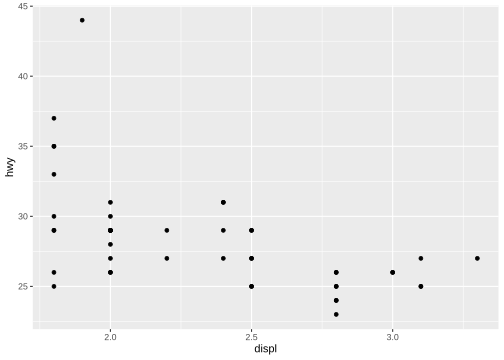
\includegraphics{rmarkdown_tutorial_files/figure-latex/unnamed-chunk-9-1.pdf}
{[}Rmd
cheatsheet{]}{[}\url{https://www.rstudio.com/wp-content/uploads/2016/03/rmarkdown-cheatsheet-2.0.pdf}{]}

\hypertarget{output-formats}{%
\subsection{Output formats}\label{output-formats}}

Rmarkdown can the generate the following document types: - pdf\_document
(requires LaTex) - word\_document - odt\_document - rtf\_document -
md\_document - github\_document

\hypertarget{how-to-generate-output-format}{%
\paragraph{How to generate output
format?}\label{how-to-generate-output-format}}

\begin{itemize}
\tightlist
\item
  change output in YAML
\item
  rmarkdown::render()
\item
  knit dropdown
\end{itemize}

\hypertarget{output-options}{%
\paragraph{output options}\label{output-options}}

check parameters associated with specific outputs and change it by
expanding output field

\hypertarget{more-output-formats}{%
\subsection{More output formats}\label{more-output-formats}}

\hypertarget{presentations-httpsrpubs.comlyong768323}{%
\paragraph{\texorpdfstring{Presentations
{[}\url{https://rpubs.com/lyong/768323}{]}}{Presentations {[}https://rpubs.com/lyong/768323{]}}}\label{presentations-httpsrpubs.comlyong768323}}

\hypertarget{dashboards-httpsrpubs.comlyong768330}{%
\paragraph{\texorpdfstring{Dashboards
{[}\url{https://rpubs.com/lyong/768330}{]}}{Dashboards {[}https://rpubs.com/lyong/768330{]}}}\label{dashboards-httpsrpubs.comlyong768330}}

\hypertarget{shiny-app-httpsluoyan-yong.shinyapps.iodemonstrate_clt}{%
\paragraph{\texorpdfstring{Shiny app
{[}\url{https://luoyan-yong.shinyapps.io/demonstrate_CLT/}{]}}{Shiny app {[}https://luoyan-yong.shinyapps.io/demonstrate\_CLT/{]}}}\label{shiny-app-httpsluoyan-yong.shinyapps.iodemonstrate_clt}}

\hypertarget{website-rmarkdownrender_site}{%
\paragraph{website
(rmarkdown::render\_site())}\label{website-rmarkdownrender_site}}

\hypertarget{graphics-for-communication}{%
\subsection{Graphics for
Communication}\label{graphics-for-communication}}

\hypertarget{labels}{%
\subsubsection{Labels}\label{labels}}

Add descriptive plot title

\begin{verbatim}
## `geom_smooth()` using method = 'loess' and formula 'y ~ x'
\end{verbatim}

\includegraphics{rmarkdown_tutorial_files/figure-latex/unnamed-chunk-11-1.pdf}

Add subtitles and/or captions

\begin{verbatim}
## `geom_smooth()` using method = 'loess' and formula 'y ~ x'
\end{verbatim}

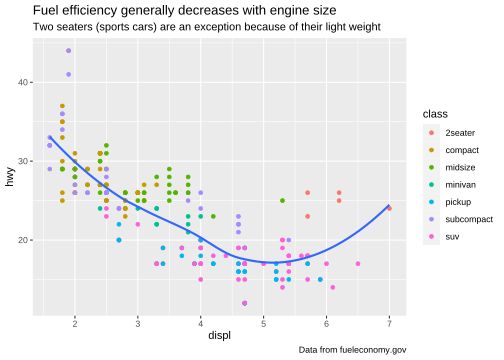
\includegraphics{rmarkdown_tutorial_files/figure-latex/unnamed-chunk-12-1.pdf}

Replace axis or legend titles with labs()

\begin{verbatim}
## `geom_smooth()` using method = 'loess' and formula 'y ~ x'
\end{verbatim}

\includegraphics{rmarkdown_tutorial_files/figure-latex/unnamed-chunk-13-1.pdf}

add math formulas with quote()

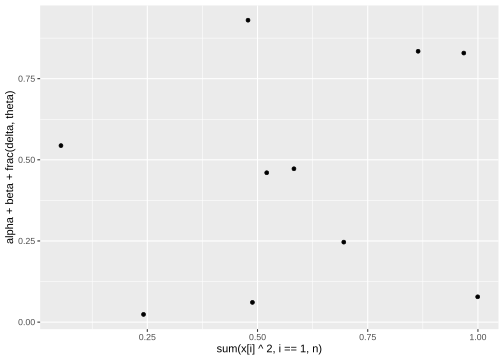
\includegraphics{rmarkdown_tutorial_files/figure-latex/unnamed-chunk-14-1.pdf}

\hypertarget{annotations}{%
\subsubsection{Annotations}\label{annotations}}

label individual observations or groups with geom\_text()

\includegraphics{rmarkdown_tutorial_files/figure-latex/unnamed-chunk-15-1.pdf}

highlight text by adding boxes with geom\_label()

\includegraphics{rmarkdown_tutorial_files/figure-latex/unnamed-chunk-16-1.pdf}

automatically adjust labels to prevent overlap using ggrepel pacakge and
add layer to highlight points

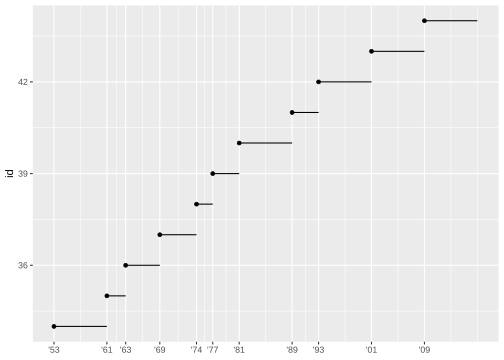
\includegraphics{rmarkdown_tutorial_files/figure-latex/unnamed-chunk-17-1.pdf}

replace legend with labels directly on plot

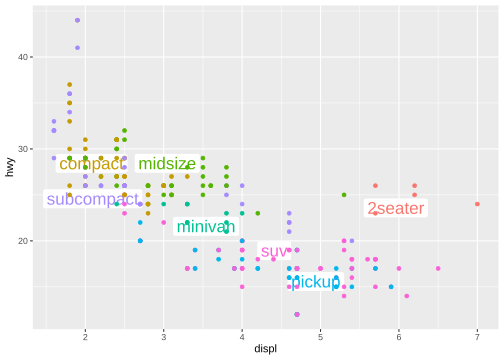
\includegraphics{rmarkdown_tutorial_files/figure-latex/unnamed-chunk-18-1.pdf}

add text in plot border with Inf and wrap text using \n or
stringr::str\_wrap()

\includegraphics{rmarkdown_tutorial_files/figure-latex/unnamed-chunk-19-1.pdf}

use vjust and hjust to adjust position of your labels or text
\includegraphics{/g/typas/Personal_Folders/Luoyan/emblR/Rmarkdown/hjust_vjust_combinations.png}

\hypertarget{scales}{%
\subsubsection{Scales}\label{scales}}

adjust your axis ticks for better visualisation, suppress labels with
NULL

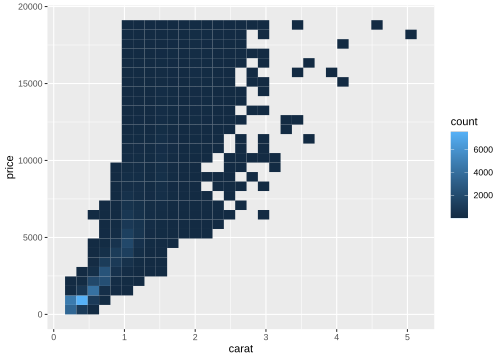
\includegraphics{rmarkdown_tutorial_files/figure-latex/unnamed-chunk-20-1.pdf}

adjust breaks especially when you have sparse data points

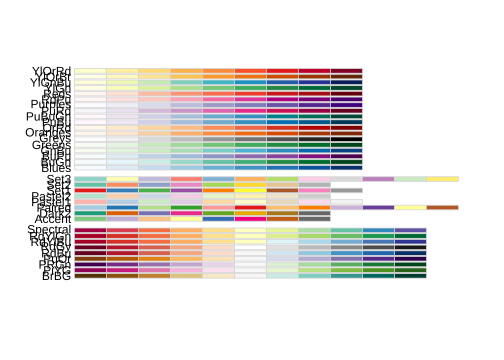
\includegraphics{rmarkdown_tutorial_files/figure-latex/unnamed-chunk-21-1.pdf}

use theme to adjust legend position

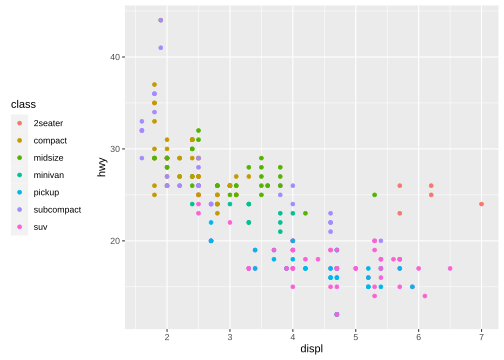
\includegraphics{rmarkdown_tutorial_files/figure-latex/unnamed-chunk-22-1.pdf}
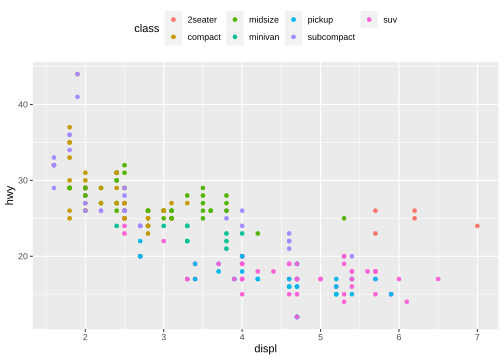
\includegraphics{rmarkdown_tutorial_files/figure-latex/unnamed-chunk-22-2.pdf}
\includegraphics{rmarkdown_tutorial_files/figure-latex/unnamed-chunk-22-3.pdf}
\includegraphics{rmarkdown_tutorial_files/figure-latex/unnamed-chunk-22-4.pdf}

use guides() to control legend display

\begin{verbatim}
## `geom_smooth()` using method = 'loess' and formula 'y ~ x'
\end{verbatim}

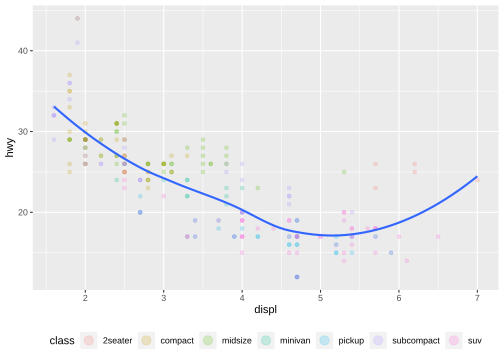
\includegraphics{rmarkdown_tutorial_files/figure-latex/unnamed-chunk-23-1.pdf}

Replace entire scale

\includegraphics{rmarkdown_tutorial_files/figure-latex/unnamed-chunk-24-1.pdf}
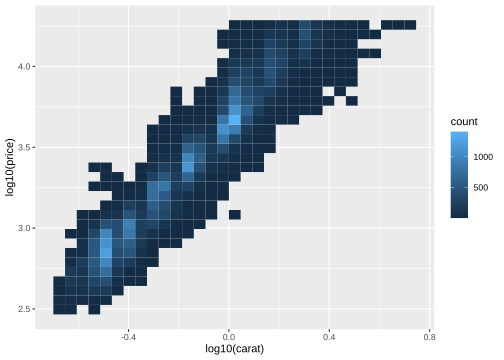
\includegraphics{rmarkdown_tutorial_files/figure-latex/unnamed-chunk-24-2.pdf}

adjusting color with RColorBrewer

\includegraphics{rmarkdown_tutorial_files/figure-latex/unnamed-chunk-25-1.pdf}

use color-blind friendly theme

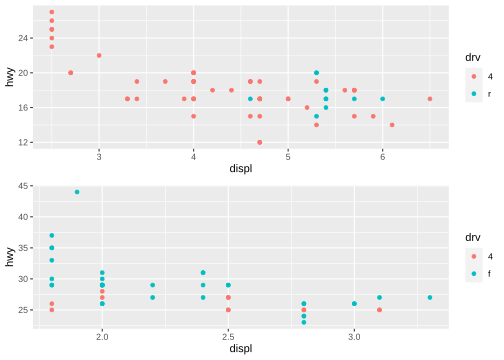
\includegraphics{rmarkdown_tutorial_files/figure-latex/unnamed-chunk-26-1.pdf}
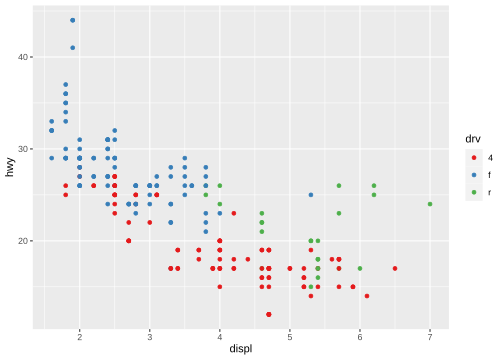
\includegraphics{rmarkdown_tutorial_files/figure-latex/unnamed-chunk-26-2.pdf}

use scale\_color\_manual to use predefined mapping between values and
colors

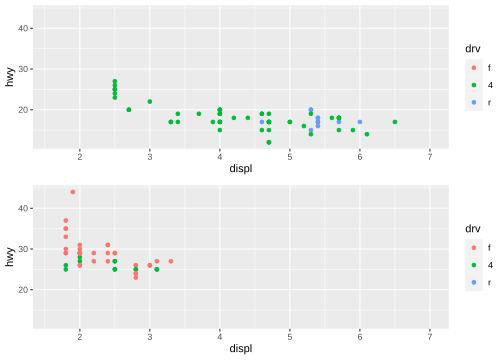
\includegraphics{rmarkdown_tutorial_files/figure-latex/unnamed-chunk-27-1.pdf}

adjust continuous color scales with scale\_color\_gradient() or
scale\_fill\_gradient() or viridis package

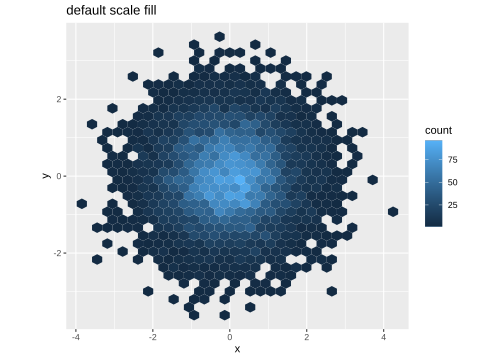
\includegraphics{rmarkdown_tutorial_files/figure-latex/unnamed-chunk-28-1.pdf}
\includegraphics{rmarkdown_tutorial_files/figure-latex/unnamed-chunk-28-2.pdf}
\includegraphics{rmarkdown_tutorial_files/figure-latex/unnamed-chunk-28-3.pdf}

\hypertarget{zooming}{%
\subsubsection{Zooming}\label{zooming}}

zoom into a plot region using coord\_cartesian

\begin{verbatim}
## `geom_smooth()` using method = 'loess' and formula 'y ~ x'
\end{verbatim}

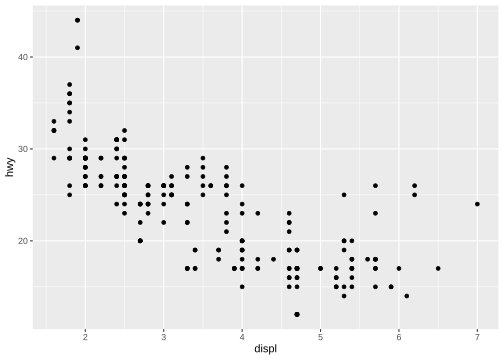
\includegraphics{rmarkdown_tutorial_files/figure-latex/unnamed-chunk-29-1.pdf}

Adjust plot limits to allow comparison on the same scale

\includegraphics{rmarkdown_tutorial_files/figure-latex/unnamed-chunk-30-1.pdf}

Expand scale of the 2nd plot so that it is comparable

\includegraphics{rmarkdown_tutorial_files/figure-latex/unnamed-chunk-31-1.pdf}

\hypertarget{themes}{%
\subsubsection{Themes}\label{themes}}

by default, there are 8 themes in ggplot2, use ggthemes to add extra
themes

\begin{verbatim}
## `geom_smooth()` using method = 'loess' and formula 'y ~ x'
\end{verbatim}

\includegraphics{rmarkdown_tutorial_files/figure-latex/unnamed-chunk-32-1.pdf}

\begin{verbatim}
## `geom_smooth()` using method = 'loess' and formula 'y ~ x'
\end{verbatim}

\includegraphics{rmarkdown_tutorial_files/figure-latex/unnamed-chunk-32-2.pdf}

\begin{verbatim}
## `geom_smooth()` using method = 'loess' and formula 'y ~ x'
\end{verbatim}

\includegraphics{rmarkdown_tutorial_files/figure-latex/unnamed-chunk-32-3.pdf}

\begin{verbatim}
## `geom_smooth()` using method = 'loess' and formula 'y ~ x'
\end{verbatim}

\includegraphics{rmarkdown_tutorial_files/figure-latex/unnamed-chunk-32-4.pdf}

\begin{verbatim}
## `geom_smooth()` using method = 'loess' and formula 'y ~ x'
\end{verbatim}

\includegraphics{rmarkdown_tutorial_files/figure-latex/unnamed-chunk-32-5.pdf}

\begin{verbatim}
## `geom_smooth()` using method = 'loess' and formula 'y ~ x'
\end{verbatim}

\includegraphics{rmarkdown_tutorial_files/figure-latex/unnamed-chunk-32-6.pdf}

\begin{verbatim}
## `geom_smooth()` using method = 'loess' and formula 'y ~ x'
\end{verbatim}

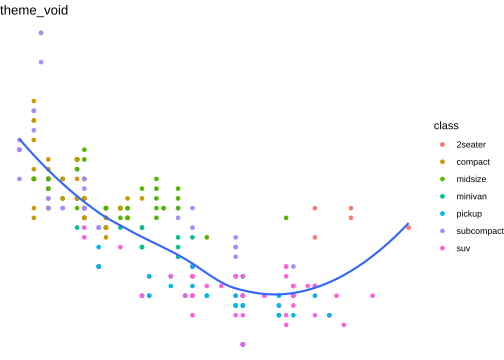
\includegraphics{rmarkdown_tutorial_files/figure-latex/unnamed-chunk-32-7.pdf}

\hypertarget{saving-your-plots}{%
\subsubsection{Saving your plots}\label{saving-your-plots}}

use ggsave or knitr

\includegraphics{rmarkdown_tutorial_files/figure-latex/unnamed-chunk-33-1.pdf}

\begin{verbatim}
## Saving 6.5 x 4.5 in image
\end{verbatim}

adjust figure sizing with fig.width or out.width for output and add
captio with fig.cap

\begin{figure}
\centering
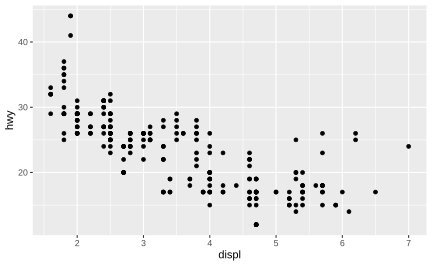
\includegraphics{rmarkdown_tutorial_files/figure-latex/unnamed-chunk-34-1.pdf}
\caption{cars plot}
\end{figure}

\end{document}
